\structure{ВЫПОЛНЕНИЕ~ДОМАШНЕГО~ЗАДАНИЯ}

1. Начальные капитальные затраты:
\[
K_n = K_c + K_b = 12,0 + 3,5 = 15,5 \, \text{млн руб.}
\]

2. Коэффициент готовности:
\[
k_r = \frac{K_n}{K_{\text{пр}}} = \frac{15,5}{20} = 0,775
\]

3. Показатель степени "b" кривой освоения:
\[
b = 0,6 - 0,5 \cdot k_r = 0,6 - 0,5 \cdot 0,775 = 0,2125
\]

4. Порядковый номер изделия, освоенного производством:
\[
    N_{\text{осв}} = \sqrt[b]{\frac{T_{\text{н}}}{T_{\text{осв}}}} = \sqrt[0,2125]{\frac{540}{120}} = \sqrt[0,2125]{4.5} \approx 1186 \, \text{изделий.}
\]

5. Продолжительность периода освоения:
\[
t_{\text{осв}} = \frac{N_{\text{осв}}}{N_{\text{мес}}} = \frac{1186}{27} \approx 44 \, \text{мес.} \approx 3,7 \, \text{лет}
\]

6. Суммарная трудоёмкость изделий, изготовленных за период освоения:
\[
T_{\text{сум}} = \frac{T_{\text{н}}}{1 - b} \left(N_{\text{осв}}^{1 - b} - 1\right) = \frac{540}{1 - 0,2125} \left(1186^{1 - 0,2125} - 1\right) \approx 180025 \, \text{н -- час}
\]

7. Максимально возможный выпуск изделий по годам периода освоения -- $N_{\text{max,год}}$. Так как $N_{\text{мес}} < 0,5 \cdot N_{\text{мес.осв}}$ $(27 < 0,5 \cdot)$, длина отрезка $OE$ будет равна:

\[
|OE| = t_{\text{осв}} \cdot \left( 1 - \frac{N_{\text{мес}}}{N_{\text{мес.осв}}} \right) = 3,7 \cdot \left( 1 - \frac{27}{60} \right) \approx 2 \, \text{года}
\]

На рисунке~\ref{fig:fig01} представлен график изменения среднемесячного выпуска изделий в период освоения. Код графика приведен в Приложении 1.

\begin{figure}
  \centering
  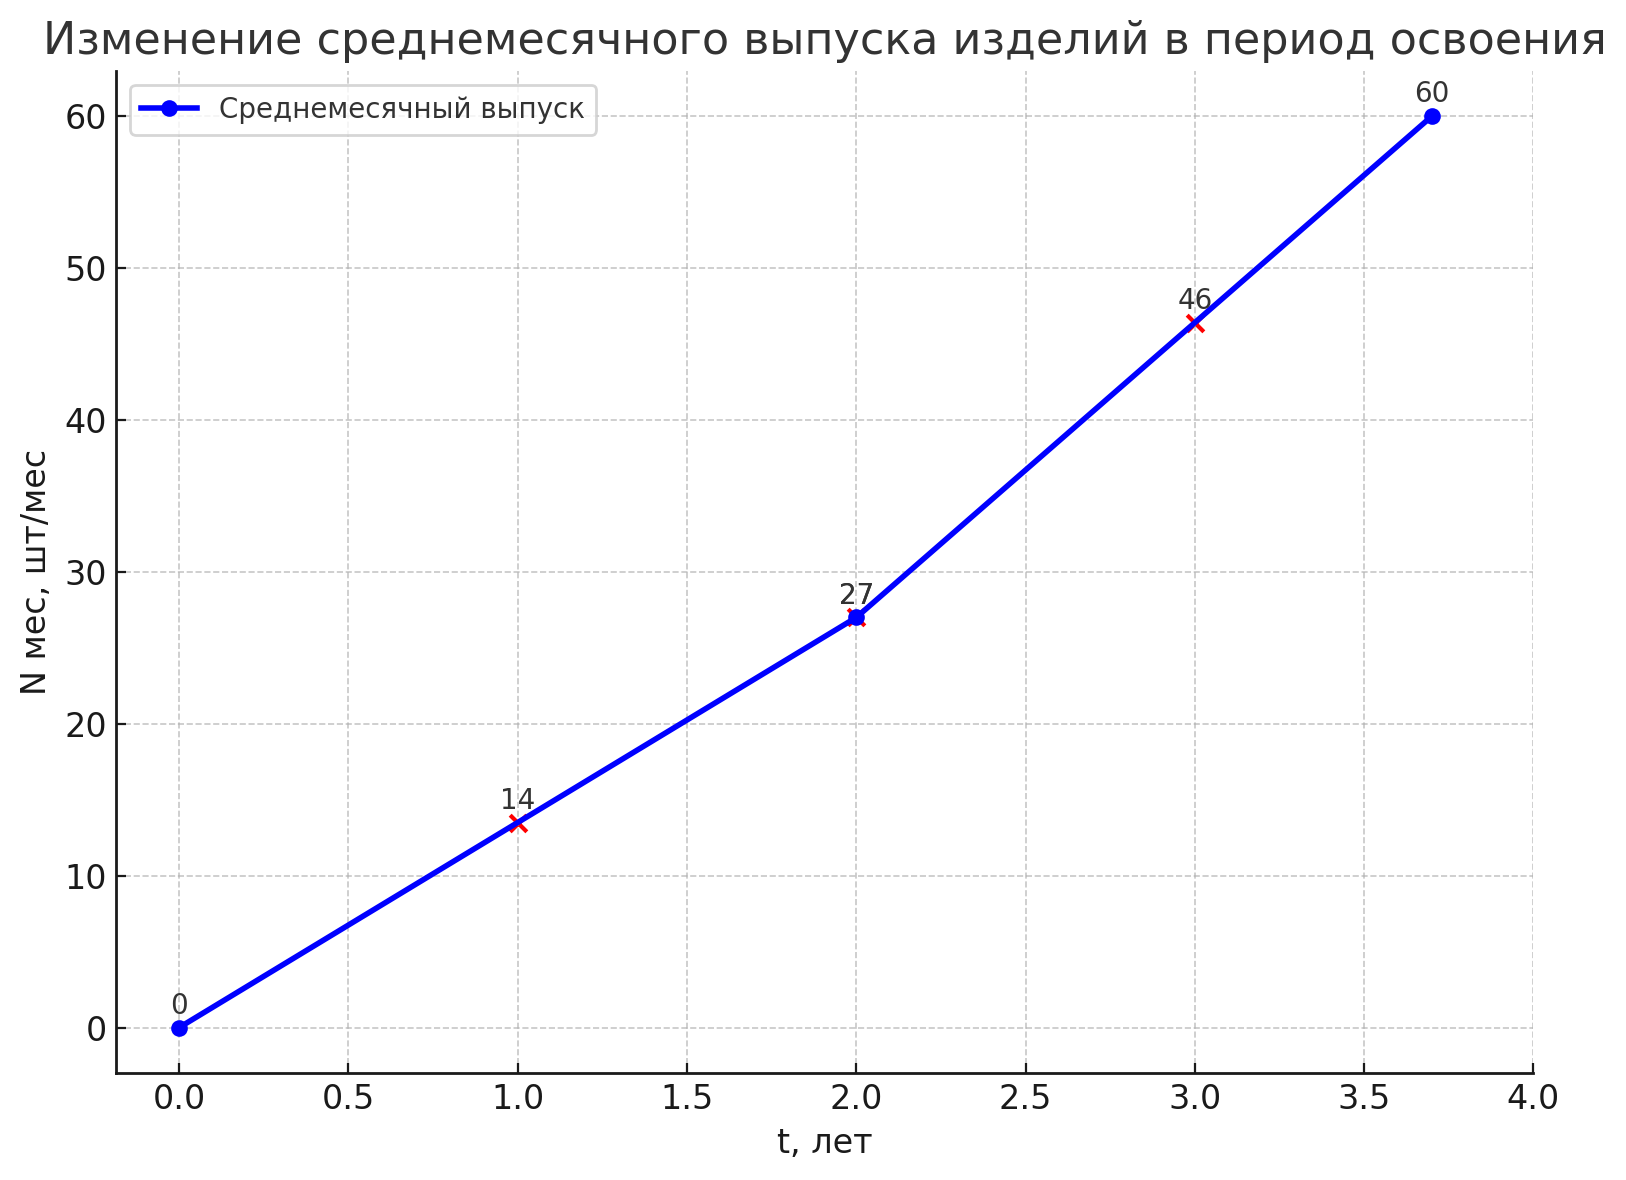
\includegraphics[scale=0.7]{inc/graph.png}
  \caption{Изменение среднемесячного выпуска изделий в период освоения}
  \label{fig:fig01}
\end{figure}

Из графика возможно определить значения $N_{\text{мес}}$, необходимые для
расчета среднемесячного выпуска в каждый год периода освоения. В итоге можно
установить порядковые номера изделий по каждому году (см. табл. 3).

\begin{table}
\caption{Порядковые номера изделий}
\begin{tabularx}{\textwidth}{|c|c|c|c|} \hline
Год освоения & $N_{\text{мес}}$, шт./мес & $N_{\text{макс.год}}$, шт./год & Порядковый номер изделий \\ \hline
1            & $\frac{0 + 14}{2} = 7$ & $7 \cdot 12 = 84$ & $1 - 84$ \\ \hline
2            & $\frac{14 + 27}{2} = 20,5$ & $20,5 \cdot 12 = 246$ & $85 - 330$ \\ \hline
3            & $\frac{27 + 46}{2} = 36,5$ & $36.5 \cdot 12 = 438$ & $331 - 768$ \\ \hline
4            & $\frac{46 + 60}{2} = 53$ & $53 \cdot 8 = 424$ & $769 - 1432$ \\ \hhline{~--~}
             & $\frac{60 + 60}{2} = 60$ & $60 \cdot 4 = 240$ &  \\ \hline
\end{tabularx}
\label{tab:tab1}
\end{table}

8. Трудоемкость изделий по годам освоения. Расчет производится по следующим формулам.

Суммарная трудоёмкость за $j$-й год:
\[
T_{\text{сум},j} = \frac{T_{\text{н}}}{1-b} \cdot \left( N_{\text{m}}^{1-b} - N_{\text{n}}^{1-b} \right)
\]
Средняя трудоёмкость за $j$-й год:
\[
T_{\text{ср},j} = \frac{T_{\text{сум},j}}{N_{\text{сум},j}} = \frac{T_{\text{сум},j}}{N_{\text{m}} - N_{\text{n}} + 1}
\]

\noindent где:
\begin{itemize}
    \item $T_{\text{н}} = 500$ — трудоёмкость первого изделия;
    \item $b$ — коэффициент снижения трудоёмкости;
    \item $N_{\text{n}}$, $N_{\text{m}}$ — порядковые номера изделий на начало и конец года.
\end{itemize}

\textbf{1-й год:}
\[
T_{\text{сум}1} = \frac{540}{1 - 0,2125} \cdot (84^{1 - 0,2125} - 1) \approx 21780 \, \text{[н-ч]}
\]
\[
T_{\text{ср}1} = \frac{21780}{84} \approx 259 \, \text{[н-ч]}
\]

\vspace{0.5cm}
\textbf{2-й год:}
\[
T_{\text{сум}2} = \frac{540}{1 - 0,2125} \cdot (330^{1 - 0,2125} - 85^{1 - 0,2125}) \approx 43313 \, \text{[н-ч]}
\]
\[
T_{\text{ср}2} = \frac{43313}{246} \approx 176 \, \text{[н-ч]}
\]

\vspace{0.5cm}
\textbf{3-й год:}
\[
T_{\text{сум}3} = \frac{540}{1 - 0,2125} \cdot (768^{1 - 0,2125} - 331^{1 - 0,2125}) \approx 62194 \, \text{[н-ч]}
\]
\[
T_{\text{ср}3} = \frac{62194}{438} \approx 142 \, \text{[н-ч]}
\]

\vspace{0.5cm}
\textbf{4-й год:}
\[
T_{\text{сум}4} = \frac{540}{1 - 0,2125} \cdot (1432^{1 - 0,2125} - 769^{1 - 0,2125}) = 81155 \, \text{[н-ч]}
\]
\[
T_{\text{ср}4} = \frac{81155}{424 + 240} \approx 122 \, \text{[н-ч]}
\]

9. Ошибки в расчётах суммарного количества изделий и их трудоёмкости

\textbf{1. Ошибка по суммарному количеству изделий ($\delta_1$):}
\[
\delta_1 = \left| \frac{N_{\text{осв}} - \sum_{j=1}^{4} N_{\text{макс.год},j}}{N_{\text{осв}}} \right| \cdot 100\%
\]
\[
\delta_1 = \left| \frac{1186 - (84 + 246 + 438 + 424 + 240)}{1186} \right| \cdot 100\% = \left| \frac{1186 - 1432}{1186} \right| \cdot 100\% \approx 21\%
\]

\vspace{0.5cm}
\textbf{2. Ошибка по трудоёмкости изделий ($\delta_2$):}
\[
\delta_2 = \left| \frac{T_{\text{сум}} - \sum_{j=1}^{4} T_{\text{сум},j}}{T_{\text{сум}}} \right| \cdot 100\%
\]
\[
\delta_2 = \left| \frac{180025 - (21780 + 43313 + 62194 + 81155)}{180025} \right| \cdot 100\% \approx 16\%
\]

10. Сопоставление максимально возможного выпуска продукции $N_{\text{макс.год}}$ и проектного объема продаж $q_{\text{пл}}$. Формирование плана производства и реализации по годам.

\begin{table}
\begin{tabular}{|c|c|c|c|c|c|}
\hline
\textbf{Год производства} & \textbf{1} & \textbf{2} & \textbf{3} & \textbf{4} & \textbf{5} \\ \hline
$N_{\text{макс.год}}$ & 84 & 246 & 438 & 644 & 720 \\ \hline
$q_{\text{пл}}$ & 350 & 580 & 600 & 500 & 450 \\ \hline
\end{tabular}
\end{table}

\textbf{1-й год:}

Спрос благоприятен, в 4 раза превышает предложение. Можно предусмотреть повышение
цены на 30\% (предельное), при этом возможный объем продаж уменьшится на 60\%:

\[
q_{\text{пр.1}} = 350 * 0,4 = 140
\]

В итоге:

\[
N_{\text{пл.год.1}} = 84 \, \text{изд.}
\]
\[
q_{\text{пр.1}} = 84 \, \text{изд.}
\]
\[
\text{Ц}_{\text{пл.1}} = 94 * 1.3 = 122,2 \, \text{тыс. руб.}
\]

\textbf{2-й год:}

Спрос благоприяен, в 2 раза превышает предложение. Можно повысить цену, обеспечив
равновесие спроса и предложения. Допустимое снижение объема продаж -- до уровня
246 изделий, т.е. на:

\[
\frac{580 - 246}{580} = 57,6\%
\]

В таком случае цену нужно повысить на 28,8\%.

В итоге:

\[
N_{\text{пл.год.2}} = 246 \, \text{изд.}
\]
\[
q_{\text{пр.2}} = 246 \, \text{изд.}
\]
\[
\text{Ц}_{\text{пл.2}} = 94 * 1.288 \approx 121 \, \text{тыс. руб.}
\]

\textbf{3-й год:}

Спрос благоприятен. Можно повысить цену, обеспечив равновесие спроса и
предложения. Допустимое снижение объема продаж -- до уровня 438 изделий, т.е. на:

\[
\frac{600 - 438}{600} = 27\%
\]

В таком случае цену нужно повысить на 13.5\%.

В итоге:

\[
N_{\text{пл.год.3}} = 438 \, \text{изд.}
\]
\[
q_{\text{пр.3}} = 438 \, \text{изд.}
\]
\[
\text{Ц}_{\text{пл.3}} = 94 * 1.135 \approx 106,7 \, \text{тыс. руб.}
\]

\textbf{4-й год:}

Две стратегии:

1. Производить столько изделий, сколько можно продать, т.е. 500 изд. При этом
выпуск продукции будет меньше максимально возможного выпуска на:

\[
\frac{644 - 500}{644} = 22\%
\]

Что приведет к росту себестоимости на $22 * k_p = 22 * 0,4 = 8.8\%$.

В итоге:

\[
N_{\text{пл.год.4}} = 500 \, \text{изд.}
\]
\[
q_{\text{пр.4}} = 500 \, \text{изд.}
\]
\[
\text{Ц}_{\text{пл.4}} = 94 \, \text{тыс. руб.}
\]

Рост себестоимости на 8.8\%

2. Снизить цену до уровня, который позволил бы повысить объем продаж до 644.
Необходимый рост объема продаж:

\[
\frac{644-500}{500} = 28.8\%
\]

Это может быть обеспечено снижением цены на $\frac{28.8}{2} = 14.4\%$.

В итоге:
\[
N_{\text{пл.год.4}} = 644 \, \text{изд.}
\]
\[
q_{\text{пр.4}} = 644\, \text{изд.}
\]
\[
\text{Ц}_{\text{пл.4}} = 94 * 0.856 = 80.5 \, \text{тыс. руб.}
\]

\textbf{5-й год:}

Две стратегии:

1. Производить столько изделий, сколько можно продать, т.е. 450 изд. При этом
выпуск продукции будет меньше максимально возможного выпуска на:

\[
\frac{720 - 450}{720} = 37.5\%
\]

Что приведет к росту себестоимости на $37.5 * k_p = 37.5 * 0,4 = 14\%$.

В итоге:

\[
N_{\text{пл.год.5}} = 450 \, \text{изд.}
\]
\[
q_{\text{пр.5}} = 450 \, \text{изд.}
\]
\[
\text{Ц}_{\text{пл.5}} = 94 \, \text{тыс. руб.}
\]

Рост себестоимости на 14\%

2. Снизить цену до уровня, который позволил бы повысить объем продаж до 720.
Необходимый рост объема продаж:

\[
\frac{720-450}{450} = 60\%
\]

Это может быть обеспечено снижением цены на $\frac{60}{2} = 30\%$.

В итоге:
\[
N_{\text{пл.год.5}} = 720\, \text{изд.}
\]
\[
q_{\text{пр.5}} = 720\, \text{изд.}
\]
\[
\text{Ц}_{\text{пл.5}} = 94 * 0.7 = 65.8 \, \text{тыс. руб.}
\]

\begin{table}
\caption{Планируемая программа производства и реализации продукции}
\begin{tabular}{|c|c|c|c|c|} \hline
\textbf{Год производства} & \begin{tabular}[c]{@{}c@{}}Планируемый \\ выпуск продукции \\ $N_{\text{пл. год}},$ изд./год\end{tabular} & \begin{tabular}[c]{@{}c@{}}Планируемый \\ объем продаж \\ $q_{\text{пл.}},$ изд./год\end{tabular} & \begin{tabular}[c]{@{}c@{}}Плановая \\ цена $\text{Ц}_{\text{пл.}},$ \\ тыс. руб.\end{tabular} & Прим. \\ \hline
1 & 84 & 84 & 122.2 & \\ \hline
2 & 246 & 246 & 121 & \\ \hline
3 & 438 & 438 & 106.7 & \\ \hline
4(1) & 500 & 500 & 94 & 8.8\% \\ \hline
4(2) & 644 & 644 & 80.5 & \\ \hline
5(1) & 450 & 450 & 94 & 14\% \\ \hline
5(2) & 720 & 720 & 65.8 & \\ \hline
\end{tabular}
\end{table}

11. Себестоимость единицы продукции, себестоимость годового выпуска, выручка от
реализации, прибыль по годам производства.

\[
    A =
M + l_{\text{час}} T_{\text{ср.i}} \cdot \left( 1 + \frac{k_{\text{ц}} + k_{\text{оп}}}{100} \right)
+ l_{\text{час}} T_{\text{ср.i}} \cdot \frac{\alpha}{100} \\
+ l_{\text{час}} T_{\text{ср.i}} \cdot \left( 1 + \frac{\alpha}{100} \right)
\cdot \frac{\beta}{100}
\]

\[
    S_{\text{ср.i}} = A \cdot \left( 1 + \frac{k_{\text{вп}}}{100} \right)
\]

\[
    S_{\text{год.i}} = S_{\text{ср.i}} \cdot N_{\text{пл.год.i}}
\]

\[
    W_{\text{год.i}} = \text{Ц}_{\text{пл.i}} \cdot N_{\text{пл.год.i}}
\]

\[
    P_{\text{год.i}} = \text{W}_{\text{год.i}} - S_{\text{год.i}}
\]

\textbf{1-й год:}

\[
    S_{\text{ср.1}} = 108.25 \,  \text{тыс.руб}
\]

\[
    S_{\text{год.1}} = 9093 \, \text{тыс.руб}
\]

\[
    W_{\text{год.1}} = 10264.8 \, \text{тыс.руб}
\]

\[
    P_{\text{год.1}} = 1171.8 \, \text{тыс.руб}
\]

\textbf{2-й год:}

\[
    S_{\text{ср.2}} = 76.576 \,  \text{тыс.руб}
\]

\[
    S_{\text{год.2}} = 18837.7  \, \text{тыс.руб}
\]

\[
    W_{\text{год.2}} = 29766 \, \text{тыс.руб}
\]

\[
    P_{\text{год.2}} = 10928.3 \, \text{тыс.руб}
\]

\textbf{3-й год:}

\[
    S_{\text{ср.3}} = 63.602 \,  \text{тыс.руб}
\]

\[
    S_{\text{год.3}} = 27857.7 \, \text{тыс.руб}
\]

\[
    W_{\text{год.3}} = 46734.6 \, \text{тыс.руб}
\]

\[
    P_{\text{год.3}} = 18875.9 \, \text{тыс.руб}
\]

\textbf{4-й год:}

\[
    S_{\text{ср.4}} =  55.969 \,  \text{тыс.руб}
\]

\textbf{1-ая стратегия:}

\[
    S_{\text{год.4}} = 27984.5 \, \text{тыс.руб}
\]

\[
    W_{\text{год.4}} = 47000 \, \text{тыс.руб}
\]

\[
    P_{\text{год.4}} = 19050.5 \, \text{тыс.руб}
\]

\textbf{2-ая стратегия:}

\[
    S_{\text{год.4}} = 36044 \, \text{тыс.руб}
\]

\[
    W_{\text{год.4}} = 51842 \, \text{тыс.руб}
\]

\[
    P_{\text{год.4}} = 15798 \, \text{тыс.руб}
\]

Стратегия 1 выгоднее, так как имеет большую прибыль - она учитывается в
дальнейших расчетах.

\textbf{5-й год:}

\[
    S_{\text{ср.5}} = 55.969 \,  \text{тыс.руб}
\]

\textbf{1-ая стратегия:}

\[
    S_{\text{год.5}} = 25186 \, \text{тыс.руб}
\]

\[
    W_{\text{год.5}} = 42300 \, \text{тыс.руб}
\]

\[
    P_{\text{год.5}} = 17114 \, \text{тыс.руб}
\]

\textbf{2-ая стратегия:}

\[
    S_{\text{год.5}} = 40297.7 \, \text{тыс.руб}
\]

\[
    W_{\text{год.5}} = 47376 \, \text{тыс.руб}
\]

\[
    P_{\text{год.5}} = 7078.3 \, \text{тыс.руб}
\]

Стратегия 1 выгоднее, так как имеет большую прибыль - она учитывается в
дальнейших расчетах.

12. Тактика возврата заемных средств.

Банковский  кредит и проценты $K_b \cdot (1 + p) = 3500 \cdot (1 + 0.08) = 3780$
тыс. руб. могут быть выплачены по результатам первого года.

13. Среднегодовая численность основных рабочих по годам производства
приведена в таблице 5 и вычисляется по формуле

\[
C_{\text{ср},j} = \frac{T_{\text{сум},j}}{F_{\text{д}} \cdot k_B} = \frac{T_{\text{сум},j}}{1935 \cdot 1} = \frac{T_{\text{сум},j}}{1935}
\]

\begin{table}
\caption{Среднегодовая численность основных рабочих}
\begin{tabular}{|c|c|c|c|c|} \hline
Год производства & $T_{\text{ср}}, \, \text{н--час}$ & $N_{\text{пл.год}}, \, \text{шт/год}$ & $T_{\text{пл.сум}}, \, \text{н--час/год}$ & $C_{\text{ср}}$ \\ \hline
1 & 259 & 84  & 21756 & 11 \\ \hline
2 & 176 & 246 & 43296 & 22 \\ \hline
3 & 142 & 438 & 62196 & 32 \\ \hline
4 & 122 & 500 & 61000 & 31 \\ \hline
5 & 122 & 450 & 54900 & 28 \\ \hline
\end{tabular}
\end{table}

14. Фонд оплаты труда основных рабочих представлен в таблице 6 и рассчитывается
(тарифный, общий) по формулам

\[
\Phi_{\text{от},j} = l_{\text{час}} \cdot T_{\text{сум},j} \, \left[ \frac{\text{руб}}{\text{год}} \right]
\]

\[
\Phi_{\text{от},j} = l_{\text{час}} \cdot T_{\text{сум},j} \cdot \left( 1 + \frac{\alpha}{100} \right) \, \left[ \frac{\text{руб}}{\text{год}} \right]
\]

соответственно.

\begin{table}
\caption{Фонд оплаты труда}
\begin{tabular}{|c|c|c|c|c|} \hline
\textbf{Год производства} & \begin{tabular}[c]{@{}c@{}}$T_{\text{пл.сум}},$ \\ н--час/год\end{tabular} & \begin{tabular}[c]{@{}c@{}}Тарифный $\Phi_{\text{от}},$ \\ тыс.руб./год\end{tabular} & \begin{tabular}[c]{@{}c@{}}Общий $\Phi_{\text{от}},$ \\ тыс.руб./год\end{tabular} \\ \hline
1 & 21756 & 2437 & 2802 \\ \hline
2 & 43296 & 4849 & 5576 \\ \hline
3 & 62196 & 6966 & 8011 \\ \hline
4 & 61000 & 6832 & 7857 \\ \hline
5 & 54900 & 6149 & 7071 \\ \hline
\end{tabular}
\end{table}

15. Сводная информация о рассчитанных выше технико-экономических показателях,
отражающих планируемый вариант освоения производства, собраны в таблице 7.

\begin{table}[h!]
\centering
\tiny % Уменьшение шрифта
\renewcommand{\arraystretch}{1.2}
\caption{Сводная таблица технико-экономических показателей}
\begin{tabular}{|c|c|c|c|c|c|c|c|c|c|c|}
\hline
\textbf{Год производства} & \begin{tabular}[c]{@{}c@{}}$N_{\text{пл.год}},$ \\ изд./год\end{tabular} & \begin{tabular}[c]{@{}c@{}}$T_{\text{ср}},$ \\ н--час\end{tabular} & \begin{tabular}[c]{@{}c@{}}$S_{\text{год}},$ \\ тыс. руб.\end{tabular} & \begin{tabular}[c]{@{}c@{}}$W_{\text{год}},$ \\ тыс. руб.\end{tabular} & \begin{tabular}[c]{@{}c@{}}$P_{\text{год}},$ \\ тыс. руб.\end{tabular} & \begin{tabular}[c]{@{}c@{}}$T_{\text{пл.сум}},$ \\ н--час/год\end{tabular} & $C_{\text{ср}}$ & \begin{tabular}[c]{@{}c@{}}Тарифный \\ $\Phi_{\text{от}},$ \\ тыс. руб./год\end{tabular} & \begin{tabular}[c]{@{}c@{}}Общий \\ $\Phi_{\text{от}},$ \\ тыс. руб./год\end{tabular} \\ \hline
1 & 84  & 259 & 9093 & 10264.8 & 1171 & 21756 & 11 & 2437 & 2802 \\ \hline
2 & 246 & 176 & 18837.7 & 29766 & 10928.3 & 53296 & 22 & 4849 & 5576 \\ \hline
3 & 438 & 142 & 27857.7 & 46734.6 & 18875.9 & 62196 & 32 & 6966 & 8011 \\ \hline
4 & 500 & 122 & 27984.5 & 47000 & 19050.5 & 61000 & 31 & 6832 & 7857 \\ \hline
5 & 450 & 122 & 25186 & 42300 & 17114 & 54900 & 28 & 6149 & 7071 \\ \hline
\end{tabular}
\end{table}
